\documentclass{article}
\usepackage[utf8]{inputenc}
\usepackage{listings}
\usepackage{color}

\usepackage[left=2cm, right=2cm, top=2cm]{geometry}
\title{IO\_URING}
\author{Dinesh Reddy}
\date{April 2023}

\usepackage{graphicx}
\graphicspath{ {../report/} }
\usepackage[colorlinks=true, allcolors=blue]{hyperref}
\usepackage{listings}

\lstset{basicstyle=\footnotesize\ttfamily,breaklines=true}
\lstset{framextopmargin=1pt,frame=lrtb}

% REMEMBER TO SUBMIT YOUR CODE AND THE OUTPUT FILE FOR STRACE

\begin{document}
\maketitle
\section{Abstract}
With Moore's Law scaling slowing, the hardware trends moved towards parallelism, necessitating the need for asynchronous 
system calls to harness the performance benefits of parallel hardware. IO\_URING is a simple-to-use 
interface copared to other existing interfaces like "aio" introduced in the Linux Kernels 5.1 and 
is being rapidly adopted for various IO applications -- network and block. In this report, 
we show the efficacy of IO\_URING in file-copy utilities by improving the performance in terms of time taken to complete the 
task by around 88\% when recursively copying files in a directory and about 80\% when copying medium-sized files of 32MB each 
and 72\% when copying large files of size 1GB.

\section{IO\_URING}

IO\_URING is an I/O interface designed to provide a more efficient way of handling I/O operations, especially in highly 
parallel workloads.

Here are some of the key advantages of IO\_URING:
\begin{itemize}
\item Zero-copy: One of the primary benefits of IO\_URING is that it allows for zero-copy I/O operations. 
Zero-copy means data can be transferred from one location to another without using multiple buffers or memory copies. 
This significantly reduces the overhead associated with copying data, improving performance and reducing overall CPU utilization.
\item Reduce system-call overhead: Another important benefit of IO\_URING is that it reduces it. In traditional I/O interfaces, 
each I/O operation requires a system call, which can be expensive regarding CPU cycles. In contrast, IO\_URING allows for batched 
requests, meaning that multiple I/O operations can be combined into a single system call. This reduces the overall overhead 
associated with I/O and improves performance.
\item Batched requests: With IO\_URING, submitting multiple I/O requests in a single batch is possible. This allows for more efficient 
use of system resources and reduces the overall latency of I/O operations. In addition, it is possible to prioritize specific 
requests within a batch, which can be useful in workloads where some requests are more critical than others.
\end{itemize}


\section{Experimetal Setup}
\subsection{System Specifications}
I used an Ubuntu20 machine running Linux Kernel version 5.4.0-146 on an Intel x86\_64 QuardCore CPU chipset of 
i5-5200U CPU @ 2.20GHz with 8GB RAM with ext4 as the underlying file system for all the experiments.

\noindent\begin{minipage}{.45\textwidth}
    \begin{lstlisting}[language=Bash, caption=Create a Virtual disk, basicstyle=\tiny]
sudo mkdir ./virtualdisk
sudo dd if=/dev/zero of=./virtualdisk/vdisk.img bs=1G count=10
sudo losetup /dev/loop40 ./virtualdisk/vdisk.img
sudo mkfs.ext4 /dev/loop40 
    \end{lstlisting}
    \end{minipage}\hfill
    \begin{minipage}{.45\textwidth}
    \begin{lstlisting}[language=Bash, caption=mount and unmount when using,frame=tlrb, basicstyle=\tiny]{Name}
sudo mount /dev/loop40 ./virtualdisk
sudo dd if=/dev/urandom of=./virtualdisk/largefile bs=1G count=1
# access the file
# ...
sudo umount virtualdisk
sudo losetup -d /dev/loop40
    \end{lstlisting}
    \end{minipage}

Though the choice of hardware doesn't explicitly expose the performance benefits of parallel hardware, we still expect some 
advantages associated with minimizing system calls and zero-copying.

We performed every experiment 5 times to minimize statistical noise.


For the experiments involving IO\_URING benefits, we used 4K blocks and a Queue Depth of 16. This choice of QUEUE\_DEPTH was 
later found in the experiments to be sufficient, and the choice of 4K needed to be more efficient. 

To ensure that the block cache doesn't impact the performance, we mount a virtual disk and access the files from the virtual disk. 
Whenever we wanted to ensure that the file was not in the page cache, we used the "fincore" utility that gives the number of 
file blocks in RAM.


\section{Understanding metrics}
\subsection{Latency}
Latency is one metric to understand the end-to-end delay of an operation to a device. Studies on this would expose the critical 
path latency and isolate the impact of payload size while copying.

As shown in Listings3, our measured latency is the time it takes for the read system call to return in the case of the 
synchronous option, and in the case of IO\_URING, it is the time for the submitted IO\_URING\_READ\_OP to appear in the 
CompletionQueue so that the "wait" call finishes. 

It should be noted that our latency is not a completion latency. The completion latency can be much higher for both io\_uring 
and synchronous operations. This latency measure would emphasize the system's responsiveness rather than the throughput. 

\begin{lstlisting}[language=C, caption=Latency of Concerned Operations shown in the Psedocode, basicstyle=\tiny]
int latency_main(int argc, char **argv) {
    fd = open("virtualdisk/largefile", O_RDONLY | O_DIRECT); // Open the file

    int block_num = opts.opt_random ? rand() % NUM_BLOCKS : 0;
    if(opts.opt_synchronous) ret = lseek(fd, block_num*BLOCK_SIZE, SEEK_SET);
    else io_uring_setup_and_init(block_num);

    gettimeofday(&submit_time, NULL); // after submitting all the request
    if(opts.opt_synchronous) ret = read(fd, read_buffer, BLOCK_SIZE);
    else{
        io_uring_submit(&ring); 
        ret = io_uring_wait_cqe(&ring, &cqe);
    }
    gettimeofday(&end_time, NULL); // End the timer
}
\end{lstlisting}

\begin{figure}
    \centering
    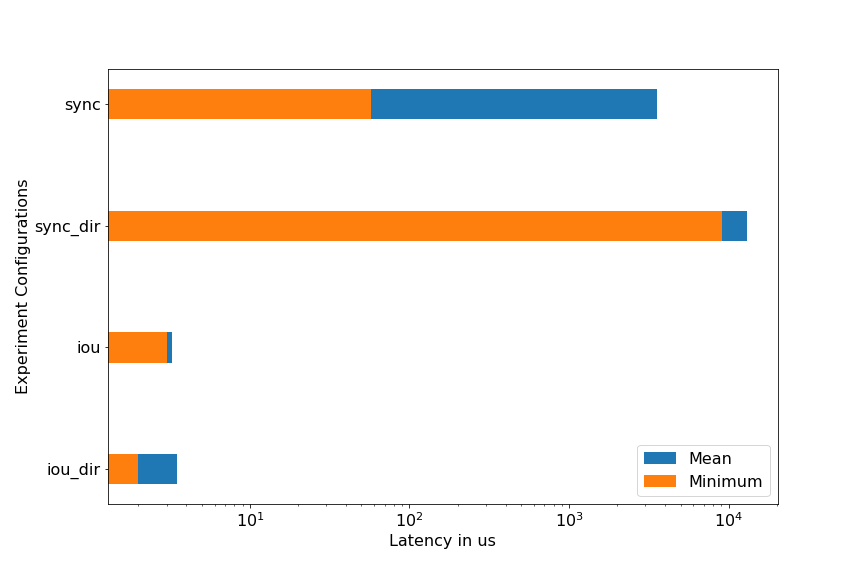
\includegraphics[scale = 0.3]{latency.png}
    \caption{4K block random read latency comparision between synchronous
    and io\_uring where
    sync\_dir: synchronous O\_DIRECT enabled access;
    sync: synchronous access;
    iou: IO\_URING access;
    iou\_dir: O\_DIRECT enabled IO\_URING access.
    }
    \label{Figure1}
\end{figure}

From Figure1. we can notice that the Latency of io\_uring is in the order of a few microseconds. 
However, the Latency of the synchronous 
read is anywhere between a few tens of microseconds to a few milliseconds. There is 3 orders of magnitude in difference. 
One possible explanation for the high variance in Latency in the case of synchronous operation is context switches. 

To see the best-case performance, we also showed the minimum time among the five experiments in the plot. We observe that even 
the minimum time for the synchronous operations is a couple of orders of magnitude higher.

It is also interesting to notice that the O\_DIRECT flag has worsened the Latency of the synchronous read, which is 
counterintuitive to our expectations since it is a zero-copy operation. Further investigation is required to understand such 
behavior. 
\subsection{IOPS}
\begin{figure}
    \centering
    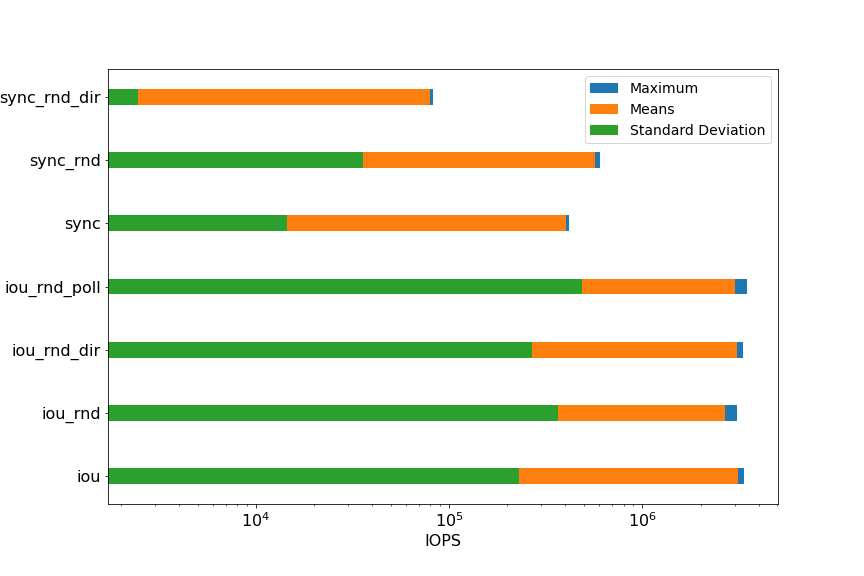
\includegraphics[scale = 0.3]{iops.png}
    \caption{4K-block random read IOPS comparision batween synchronous 
    and io\_uring where
    sync\_rand\_dir: synchronous random O\_DIRECT enabled access;
    sync\_rnd: synchronous random access;
    sync: synchronous sequential access;
    iou: IO\_URING sequential access;
    iou\_rnd: IO\_URING random access;
    iou\_rnd\_dir: O\_DIRECT enabled IO\_URING random access;
    iou\_rnd\_poll: POLLING enabled IO\_URING random access
    }
    \label{Figure2}
\end{figure}
The number of Input Output Operations per Second is defined as 
\href{IOPS}{https://en.wikipedia.org/wiki/IOPS}. 
It captures performance regarding the number of operations 
seen from userspace. We compared the performance of read operations of 4K block size while accessing a 
large file of 1GB between the 
synchronous and asynchronous version using IO\_URING with different options concerning sequential vs random, with or without 
O\_DIRECT flag set, the impact of POLLING for IO\_URING. The results are plotted in Figure 2.

From figure2, the throughput of the IO\_URING is 3x that of the synchronous indicating the efficacy of using asynchronous I/O than 
synchronous I/O. While this is much lesser than what we observed in the case of "Latency," it is still significant. 

As expected, sequential read performance is higher than random read for synchronous operations. Interestingly, in the case of 
IO\_URING, the throughput of random access is slightly higher (or insignificant). This again requires further investigation to 
determine the reasons.

The impact of POLLING is contrary to our expectation of increased throughput. We used both IORING\_SETUP\_IOPOLL and IORING\_SETUP\_SQPOLL flags 
while opening the files. IORING\_SETUP\_IOPOLL is used to enable the io-polling mechanism in io\_uring. With this flag, the kernel 
will use a busy-wait loop to poll for completions instead of relying on an eventfd-based notification mechanism. This can improve 
the application's performance by reducing the overhead of system calls.

On the other hand, IORING\_SETUP\_SQPOLL is used to enable the submission queue polling mechanism. With this flag, the kernel will 
periodically poll the submission queue for new requests instead of waiting for an eventfd-based notification. This can improve 
the application's performance by reducing the submission latency and reducing the overhead of system calls. From the plot, neither 
of the mechanisms impacted the performance.


\subsection{Completion Time}
With the amount of data to be copied the same, the total time taken to copy a large file captures the overall throughput of the 
utility. We use this metric to measure the copy utilities' performance on various file size benchmarks. 

We used the "user + system" time and ignored the real-time since it involves influence from the external environment and is often 
not a reliable metric. We noted that "real" time is much higher than "user + system" time. This was also observed in some of our 
experiments. In analyzing further, we concluded that the close system call is responsible for the increase (it takes a lot of time 
to return). However, we are still determining the exact reason for such behavior. One possible guess is that the metadata 
associated with the IO\_URING in the kernel space took extra time to clean up.


\section{Performance Tuning for IO\_URING}
\subsection{Queue Depth}
In the first experiment, with a constant BLOCK\_SIZE (4K), we sweeped across various QUEUE\_DEPTHS ranging from 1 to 256, 
multiplying with 2 each time. Here, we used IOPS as the metric. 

From the figure, we can note that IOPS increases exponentially with QUEUE\_DEPTHS for smaller QUEUE\_DEPTHS and asymptotes at 
higher QUEUE\_DEPTHS. From the plot, we can also note that after a QUEUE\_DEPTH of 16, there is little to no improvement. We 
believe that the underlying hardware limitations are causing this asymptotic behaviour.

Furthermore, we can also observe random access slightly less performant than sequential accesses, 
consistent with previous observation when analyzing the performance 
difference for a fixed QUEUE\_DEPTH in Figure2 as represented by rectangles “iou\_rnd” and “iou.”

\begin{figure}
    \centering
    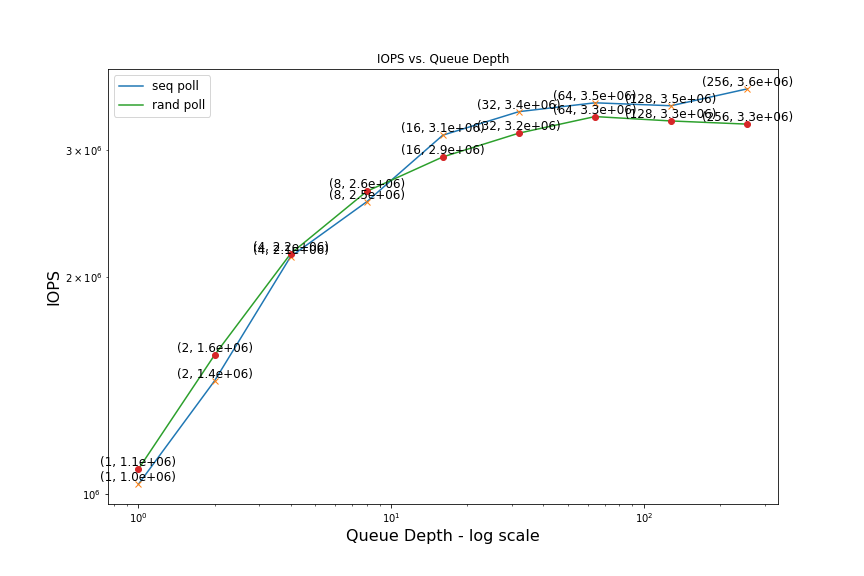
\includegraphics[scale = 0.4]{queue_depth.png}
    \caption{Impact of Queue Depth for POLLED IO\_URING while performing 4K block random reads in terms of 
    IOPS comparing sequential and random access for QUEUE\_DEPTHS ranging from 1 to 256.}
    \label{Figure3}
\end{figure}

\subsection{Block Size}
\begin{figure}
    \centering
    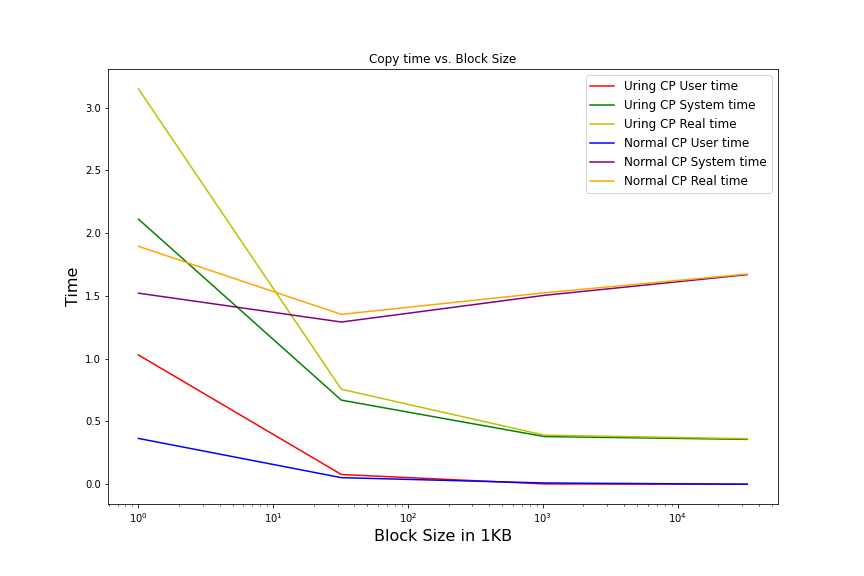
\includegraphics[scale = 0.4]{cp_bs.png}
    \caption{IO\_URING copy real, system, and user time for block sizes of 1KB to 32MB when copying 
    1GB file with a QUEUE\_DEPTH of 16.}
    \label{Figure5}
\end{figure}

\begin{figure}
    \centering
    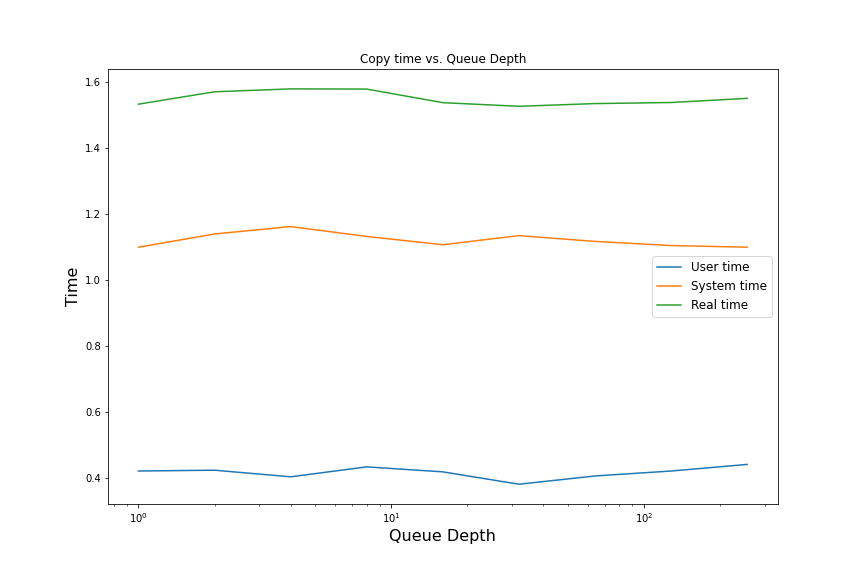
\includegraphics[scale = 0.4]{cp_qd.png}
    \caption{IO\_URING copy completion-time comparision for copying a 1GB file with across BLOCK\_SIZES 
    of 1KB, 32KB, 1MB and 32MB with QUEUE\_SIZES ranging from 1 to 256.}
    \label{Figure4}
\end{figure}

Undrestanding the impact of BLOCK\_SIZE requires an experiment invole a throughput metric — IOPS and latency are not sufficient. 
Hence, we used completion time as the metric to analyze the impact. We experimented with 4 different blocks sizes, 1KB, 32KB, 
1MB, and 32MB for this.

From the plot, we can notice that the throughput increases with BLOCK\_SIZE. The rate of change is similar to that of the 
QUEUE\_DEPTH, it improves exponentially for smaller BLOCK\_SIZE and little to none with larger BLOCK\_SIZES. We can also see that 
the decrease in time decreases with the increasing block sizes, i.e., the decrease is much smaller when BLOCK\_SIZE increases 
from 32KB to 1MB and even less from 1MB to 32MB.

We can also note from Figure4 that the user time is almost negligible compared to system time. This is expected since, we are 
not doing any effective work in user space, especially when the BLOCK\_SIZE is large, most of the time is spent in the kernel 
interacting with File System subsystem. 

\section{Evaluation}
In this section, we analyze the performance of our main utility by comparing it with system copy utility for various workloads.

Based on Figure5, we chose BLOCK\_SIZE of 32MB and QUEUE\_DEPTH of 16 for our experiments comparing uring-cp and system-cp 
utilities. 

In this experiment, we use file sizes from 1KB, 32KB, 1MB, 32MB and 1GB to capture diverse file sizes.

From the plot, we can notice that uring-cp consistently outperformed system-cp utility. As the file size increases, \% improvement 
in throughput increases from 14\% to 81\% at 32MB file sizes and slightly reduces to 72\% for 1GB files. 
The improvement is the least for 1KB file sizes because of the overhead associated with uring infrastructure relative to the 
actual data transfer. 

\begin{figure}
    \centering
    
\includegraphics[scale = 0.6]{cp_perf_compare.png}
    \caption{File Copy completion-time comparison between uring-cp and system-cp for file sizes
    1KB, 32KB, 1MB, 32MB, and 1GB when IO\_URING's BLOCK\_SIZE is 32MB and QUEUE\_DEPTH is 16.}
    \label{Figure6}
\end{figure}

\begin{table}
\centering
\begin{tabular}{|c|c|c|c|c|c|c|c|}

    \hline
    file\_size & user\_u & system\_u & user\_s & system\_s & io\_uring & system\_cp & percent decrement\\
    \hline
    1KB    &   0.0015  & 0.0000 &0.00125 &  0.0005  & 0.0015 &  0.00175 &14.28 \\
    \hline
    32KB   &   0.0010  & 0.0000 &0.00100 &  0.0010  & 0.0010 &  0.00200 &50.00 \\
    \hline
    1MB    &   0.0016  & 0.0004 &0.00140 &  0.0026  & 0.0020 &  0.00400 &50.00 \\
    \hline
    32MB   &   0.0020  & 0.0080 &0.00160 &  0.0518  & 0.0100 &  0.05340 &\textbf{81.27} \\
    \hline
    1GB    &   0.0018  & 0.3432 &0.00800 &  1.2556  & 0.3450 &  1.26360 &72.69 \\
    \hline

\end{tabular}
\caption{\label{tab:widgets}A table of Execution times in terms of user and system times for uring-cp('\_u') 
and system-cp('\_s'); completion times under 'io\_uring' and 'system\_cp'; percentage decrement under 
'percent decrement' columns.}
\vspace{0.5cm}
\end{table}

\begin{figure}
    \centering
    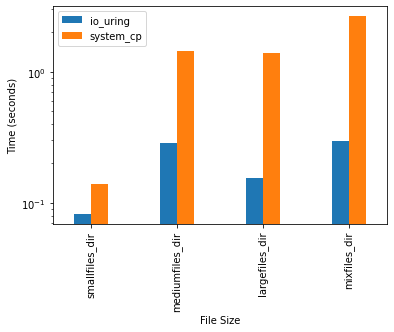
\includegraphics[scale = 0.6]{cp_perf_recursive_compare.png}
    \caption{Recursive File Copy Completion times comparison between uring-cp and system-cp for directories containing, 
    smallfiles\_dir - 1000 32KB files; 
    mediumfiles\_dir - 1000 1MB files; 
    largefiles\_dir - 32 32MB files; 
    mixfiles\_dir - 50 1KB files, 50 32KB files, 50 1MB files, and 50 32MB files.}
    \label{Figure7}
\end{figure}

\begin{table}
\centering
\begin{tabular}{|c|c|c|c|c|c|c|c|c|}

    \hline
    file\_size & user\_u & system\_u & user\_s & system\_s & io\_uring & system\_cp & percent decrement\\
    \hline                                                                                        
    smallfiles\_dir  &0.01125 & 0.07125& 0.0230 &  0.1160  & 0.0825 &   0.1390  &  40.64\\
    \hline                                                                                        
    mediumfiles\_dir &0.01880 & 0.26660& 0.0394 &  1.3986  & 0.2854 &   1.4380  &  80.15\\
    \hline                                                                                        
    largefiles\_dir  &0.00140 & 0.15260& 0.0128 &  1.3774  & 0.1540 &   1.3902  &  \textbf{88.92}\\
    \hline                                                                                        
    mixfiles\_dir    &0.00380 & 0.29140& 0.0326 &  2.6320  & 0.2952 &   2.6646  &  \textbf{88.92}\\
    \hline                                                                                        
     
\end{tabular}
\caption{\label{tab:widgets}A table of Execution times of recursive copy 
in terms of user and system times for uring-cp('\_u') 
and system-cp('\_s'); completion times under 'io\_uring' and 'system\_cp'; percentage decrement under 
'percent decrement' columns.}
\vspace{0.5cm}
\end{table}


In case of recursive file copy, the performance improvement is even higher for large file sizes of 32MB. This higher improvement 
compared to a single file is contrary to my expectation of either equal or slightly lower since my implementation is crude in 
sequentially copying each file asynchronously. In other words, a new file is started only after the previous file is completely 
copied.

We settled down with crude implementation owing to the complex copy of single file. Making it asynchronous across multiple files 
requires opening multiple files simultaneously, tracking individual file progress while aiming to improve performance. Besides, 
we already know that our HardDisk doesn’t support paralled reads at hardware level unlike nVME enabled Harddisks. This discouraged 
me against implementing multiple file copy simultaneously.


\section{Conclusion}
IO\_URING is a suitable interface in Linux Kernel to implement asynchronous I/O. Though it is more complicated than the 
asynchronous versions, it’s advantages associated with performance improvements are significant and a large class of applications 
involving I/O in the increasingly parallel hardware settings can be accelerated.

\section{Referances}



Please find the code at my git repo \href{git@github.com:chintadinesh/adv\_os-project.git}{git@github.com:chintadinesh/adv\_os-project.git}.

\href{https://www.phoronix.com/news/Linux-io\_uring-Fast-Efficient}{https://www.phoronix.com/news/Linux-io\_uring-Fast-Efficient}

\href{https://lwn.net/Articles/776703/}{https://lwn.net/Articles/776703/}

\href{https://kernel.dk/io\_uring.pdf}{https://kernel.dk/io\_uring.pdf}

\href{https://lwn.net/Articles/776703/https://git.kernel.dk/cgit/fio/plain/t/io\_uring.c}{https://lwn.net/Articles/776703/https://git.kernel.dk/cgit/fio/plain/t/io\_uring.c}

\href{https://lwn.net/Articles/221913/}{https://lwn.net/Articles/221913/}

\href{https://lwn.net/Articles/259068/}{https://lwn.net/Articles/259068/}

\href{https://lore.kernel.org/linux-block/20190116175003.17880-1-axboe@kernel.dk/}{https://lore.kernel.org/linux-block/20190116175003.17880-1-axboe@kernel.dk/}

\href{https://developers.mattermost.com/blog/hands-on-iouring-go/}{https://developers.mattermost.com/blog/hands-on-iouring-go/}

\href{https://lwn.net/Articles/810414/}{https://lwn.net/Articles/810414/}

\href{https://kernel-recipes.org/en/2019/talks/faster-io-through-io\_uring/}{https://kernel-recipes.org/en/2019/talks/faster-io-through-io\_uring/}

\href{https://lwn.net/Articles/776703/}{https://lwn.net/Articles/776703/}

\href{https://kernel.dk/axboe-kr2022.pdf}{https://kernel.dk/axboe-kr2022.pdf}

\href{https://git.kernel.org/pub/scm/linux/kernel/git/torvalds/linux.git/tree/io\_uring}{https://git.kernel.org/pub/scm/linux/kernel/git/torvalds/linux.git/tree/io\_uring}

\end{document}